\subsubsection{Volume Infused Fluid Mount Clamp Design}

The drawings below outline the fluid infusion mount, one part is required. The part is fixed to the end of the fluid infusion load cell and allows the infusion bag to be supported and weighed.
The two through holes allow bolts to pass through the part to fix the loadcell to the clamp. The upright cylinder/hook acts as the point to fix the infusion fluid bag, it should be made sufficiently strong to hold a minimum of 1.25 kg.


\begin{figure}[h]
    \centering
    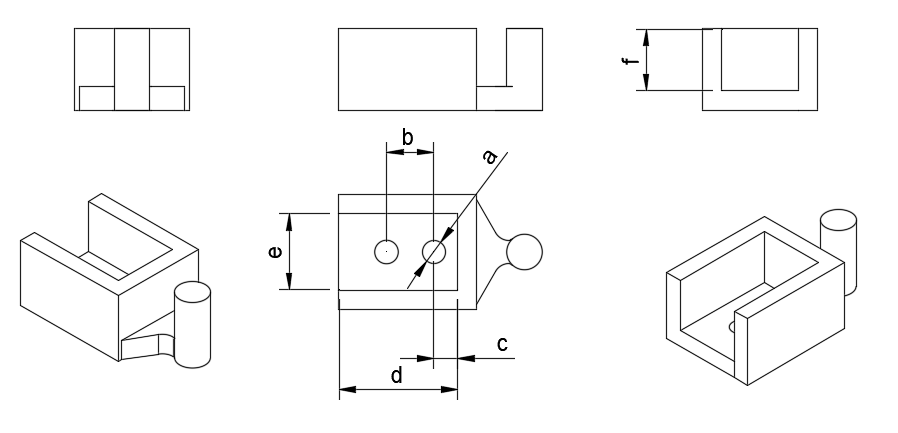
\includegraphics[width=0.7\textwidth]{Figures/SupportDrawings/vi_fluid_bag_mount_drawing.png}
    \caption{Volume Infused Fluid Mount Clamp Drawings}
    \label{fig:vimountclampdrawing}
  \end{figure}


  \begin{enumerate}
    \item[a)] The diameter of the upright stand/trolley + \textgreater\ 4mm
    \item[a)]	The bolt diameter used by the loadcell + \textgreater\ 1mm
    \item[b)]	The distance between the centre points of the two tapped holes at each end of the loadcell
    \item[c)]	The distance between the centre points loadcells outermost hole and the end of the loadcell + 1mm
    \item[d)]	Distance from the end of the loadcell to the innermost holes edge + \textgreater\ 5mm
    \item[e)]	The width of the loadcell + 4mm
    \item[f)]	Height of the loadcell

  \end{enumerate}

